\let\negmedspace\undefined
\let\negthickspace\undefined
\documentclass[journal]{IEEEtran}
\usepackage[a5paper, margin=10mm, onecolumn]{geometry}
%\usepackage{lmodern} % Ensure lmodern is loaded for pdflatex
\usepackage{tfrupee} % Include tfrupee package

\setlength{\headheight}{1cm} % Set the height of the header box
\setlength{\headsep}{0mm}     % Set the distance between the header box and the top of the text

\usepackage{gvv-book}
\usepackage{gvv}
\usepackage{cite}
\usepackage{amsmath,amssymb,amsfonts,amsthm}
\usepackage{algorithmic}
\usepackage{graphicx}
\usepackage{textcomp}
\usepackage{xcolor}
\usepackage{txfonts}
\usepackage{listings}
\usepackage{enumitem}
\usepackage{mathtools}
\usepackage{gensymb}
\usepackage{comment}
\usepackage[breaklinks=true]{hyperref}
\usepackage{tkz-euclide} 
\usepackage{listings}
% \usepackage{gvv}                                        
\def\inputGnumericTable{}                                 
\usepackage[latin1]{inputenc}                                
\usepackage{color}                                            
\usepackage{array}                                            
\usepackage{longtable}                                       
\usepackage{calc}                                             
\usepackage{multirow}                                         
\usepackage{hhline}                                           
\usepackage{ifthen}                                           
\usepackage{lscape}
\begin{document}

\bibliographystyle{IEEEtran}
\vspace{3cm}

\title{9.4.23}
\author{EE25BTECH11011 - Navya}
% \maketitle
% \newpage
% \bigskip
{\let\newpage\relax\maketitle}

\renewcommand{\thefigure}{\theenumi}
\renewcommand{\thetable}{\theenumi}
\setlength{\intextsep}{10pt} % Space between text and floats
\textbf{Question}:\\
Find the roots of the quadratic equation graphically.
\begin{align}
6x^2 - x - 2 = 0
\end{align}


\textbf{Solution}:\\
\begin{align}
y = 6x^2 - x - 2
\end{align}

This equation can be represented as the conic:
\begin{align}
\vec{x}^T\vec{V}\vec{x} + 2\vec{u}^T\vec{x} + f = 0
\end{align}
where
\begin{align}
\vec{V} = \myvec{6 & 0 \\ 0 & 0}, \quad 
\vec{u} = \myvec{-\tfrac{1}{2} \\ 0}, \quad 
f = -2
\end{align}

To find the roots, we find the points of intersection of the conic with the x-axis:
\begin{align}
\vec{x} = \vec{h} + k_i\vec{m}    
\end{align}
\begin{align}
\vec{h}=\myvec{0 \\ 0}, \quad \vec{m} = \myvec{1 \\ 0}
\end{align}

Substitute into the conic equation:
\begin{align}
(\vec{h} + k_i \vec{m})^{\top} \vec{V} (\vec{h} + k_i \vec{m}) 
+ 2\vec{u}^{\top} (\vec{h} + k_i \vec{m}) + f = 0
\end{align}

This simplifies to a quadratic in \( k_i \):
\begin{align}
k_i^2 \vec{m}^T \vec{V} \vec{m} 
+ 2k_i \vec{m}^T (\vec{V}\vec{h} + \vec{u}) 
+ g(\vec{h}) = 0
\end{align}

Now substituting the values:
\begin{align}
k_i = 
\frac{ -\vec{m}^T(\vec{V}\vec{h} + \vec{u}) 
\pm \sqrt{ [\vec{m}^T(\vec{V}\vec{h} + \vec{u})]^2 
- \vec{m}^T\vec{V}\vec{m} \cdot g(\vec{h}) } }
{\vec{m}^T \vec{V} \vec{m}}
\end{align}

\begin{align}
\Rightarrow 
k_i = 
\frac{ -(-\tfrac{1}{2}) 
\pm \sqrt{ (-\tfrac{1}{2})^2 - 6(-2) } }{6}
= 
\frac{ \tfrac{1}{2} \pm \sqrt{ \tfrac{1}{4} + 12 } }{6}
= 
\frac{ \tfrac{1}{2} \pm \tfrac{7}{2} }{6}
\end{align}

\begin{align}
\Rightarrow 
k_1 = \frac{4}{6} = \frac{2}{3}, 
\quad 
k_2 = \frac{-3}{6} = -\frac{1}{2}
\end{align}

Hence, the real roots are:
\begin{align}
\vec{x}_1 = \myvec{\tfrac{2}{3} \\ 0}, 
\quad 
\vec{x}_2 = \myvec{-\tfrac{1}{2} \\ 0}
\end{align}

\begin{figure}[h!]
    \centering
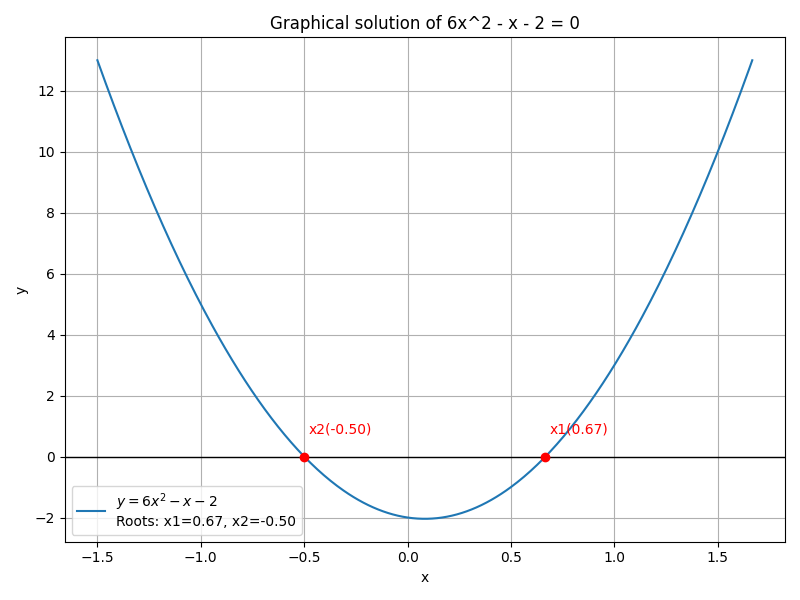
\includegraphics[width=0.8\textwidth]{figs/fig15.png}
    \label{fig:division}
\end{figure}


\end{document}